\section{Results}\label{sec:results}

\subsection{Genome comparison}

\begin{table}[H]
    \centering
    \small
    \begin{tabular}{lr}
\hline
MN908947.3 (Wuhan) length & 29903 \\
MT106054.1 (Texas) length & 29882 \\
$|LCS|$ & 29875 \\
similarity $|LCS| / \max(n, m)$ & 0.99906 \\
substituted positions & 6 \\
\quad synonymous & 3 \\
\quad non-synonymous & 3 \\
\quad outside coding regions & 0 \\
insertions / deletions / complex & 1 / 2 / 0 \\
Hirschberg time (alignment) & 3.9 s \\
full DP table memory (not run) & 3.6 GB \\
\hline
\end{tabular}
    \caption{Wuhan 2019 versus Texas 2020 by longest common subsequence.}
    \label{tab:genome}
\end{table}

\ph{What the number means. Main idea: $|LCS| = 29\,875$ against lengths 29\,903 and 29\,882 gives a similarity of 0.99906; the LCS counts symbols that can be kept in order in both genomes, so $n - |LCS| = 28$ symbols of Wuhan and $m - |LCS| = 7$ of Texas have no partner. Limitation to state: the LCS ignores locality, a scattered set of matches and a contiguous block score the same, which is why the gap analysis is needed to say where the differences are.}

\begin{table}[H]
    \centering
    \small
    \begin{tabular}{rrcclcl}
\hline
Wuhan pos & Texas pos & base & region & codon & amino acid & effect \\
\hline
8782 & 8782 & C$\to$T & QHD43415\_4 & AGC$\to$AGT & S$\to$S & synonymous \\
18603 & 18603 & T$\to$C & QHD43415\_13 & CAT$\to$CAC & H$\to$H & synonymous \\
18975 & 18975 & T$\to$A & QHD43415\_13 & GTT$\to$GTA & V$\to$V & synonymous \\
19175 & 19175 & A$\to$C & QHD43415\_13 & GAT$\to$GCT & D$\to$A & non-synonymous \\
27925 & 27925 & C$\to$T & QHD43422 & ACA$\to$ATA & T$\to$I & non-synonymous \\
28144 & 28144 & T$\to$C & QHD43422 & TTA$\to$TCA & L$\to$S & non-synonymous \\
\hline
\end{tabular}
    \caption{Substitutions between the two genomes (1-based positions) and their effect on the encoded amino acid.}
    \label{tab:mutations}
\end{table}

\begin{figure}[H]
    \centering
    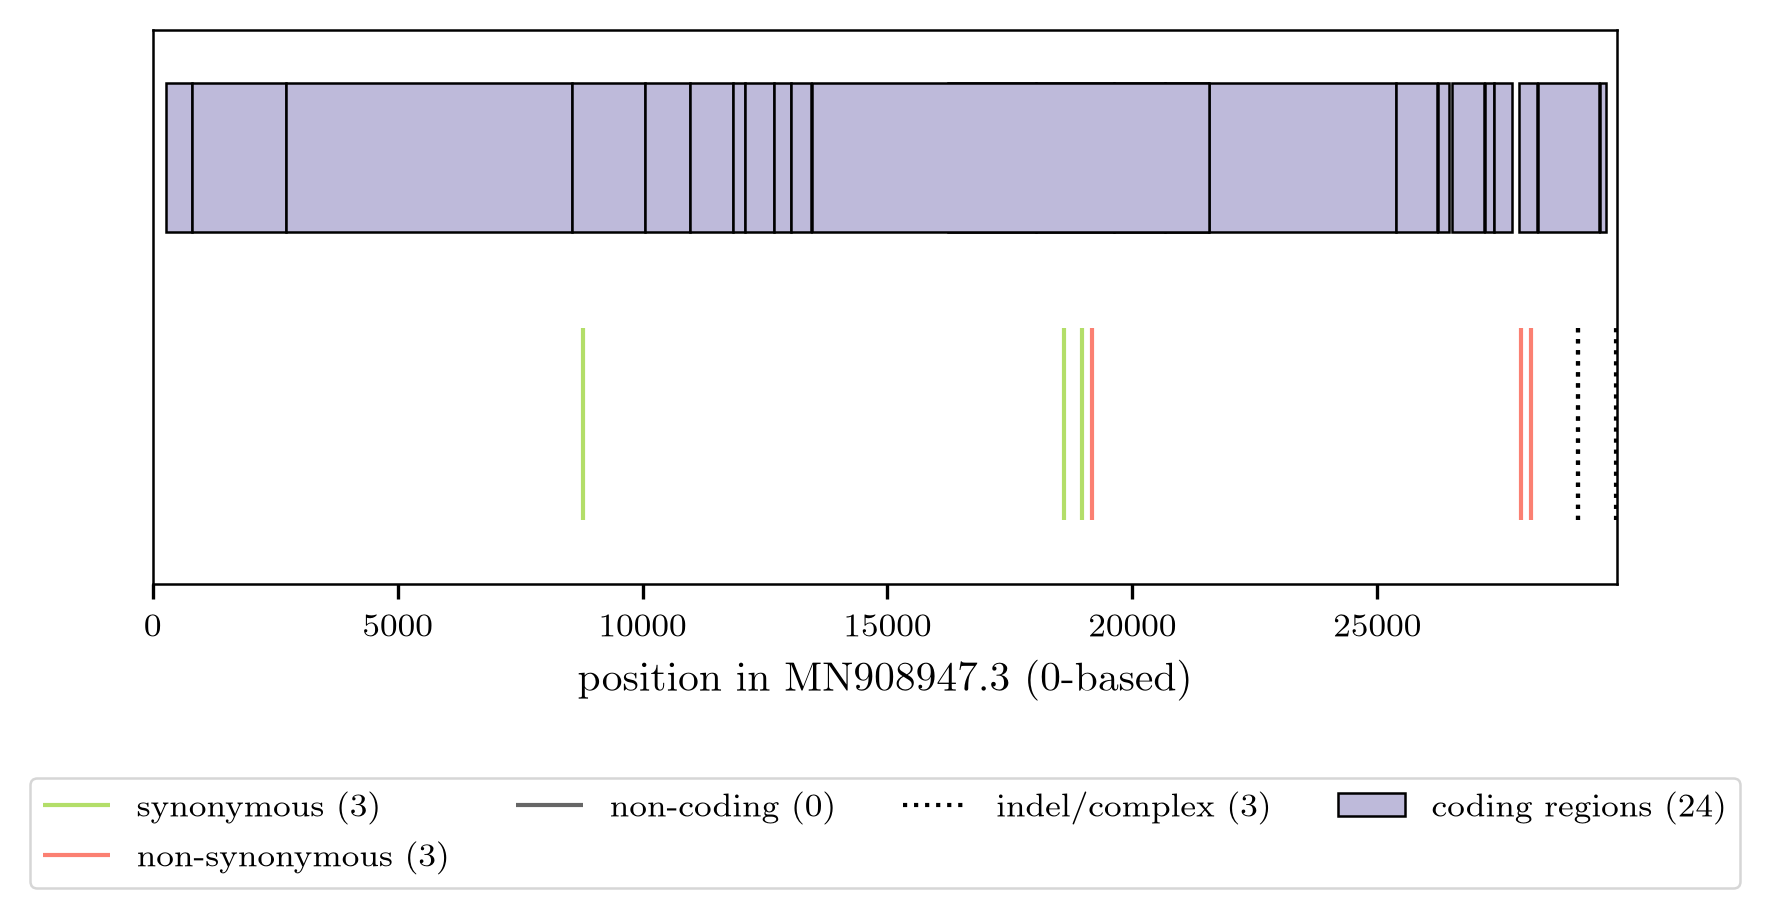
\includegraphics[width=0.72\textwidth]{fig_mutation_map}
    \caption{Position of every difference along the Wuhan genome, with the coding regions located by backtracking.}
    \label{fig:mutations}
\end{figure}

\ph{Reading Table~\ref{tab:mutations} and Figure~\ref{fig:mutations}. Main idea: six substitutions, three synonymous and three non-synonymous; the non-synonymous ones are D$\to$A in QHD43415\_13 and two in QHD43422 (T$\to$I, L$\to$S). The three indels are all after position 29\,000: a 21-nucleotide run of A missing from the Texas record, which is the poly-A tail (how far the sequencing read, not a mutation), and an insertion plus a deletion three positions apart near 29\,091 that is really one more substitution, C$\to$T at 29\,095: the LCS has no substitution operation, and when the changed base equals its neighbour (Wuhan \texttt{GCTTTCGG}, Texas \texttt{GCTTTTGG}) an indel pair and a substitution give the same LCS length, so the traceback may return either. This is the main limitation of using the LCS as a diff. Note that two substitutions fell outside the three gene files and could only be classified after backtracking located QHD43422.}

\subsection{Search, greedy, backtracking, branch and bound, palindromes}

\ph{One paragraph per technique, numbers from the appendix tables. Search: all three genes found at exactly the header coordinates (ORF1ab at 266, S at 21\,563, M at 26\,523, 1-based), and in the Texas genome S and M are found intact while ORF1ab is not, consistent with the substitutions in Table~\ref{tab:mutations}. Greedy: 187 candidate ORFs, 8 selected, S and M recovered exactly, ORF1a and ORF1b as the two large pieces; lowering the threshold to 30 codons makes greedy pick 53 small ORFs covering 30\% of the genome and none of the known genes, because the objective is the count (Table~\ref{tab:orfs}, Figure~\ref{fig:orf}). Backtracking: 23 of 24 proteins located over their full length with a few dozen nodes each; the exception, QHD43415\_11, matches exactly 9 amino acids from position 13\,441, that is, up to nucleotide 13\,468, the ribosomal frameshift, so the algorithm found the biology rather than failing (Table~\ref{tab:proteins}). Branch and bound: for $k = 8$, $d = 1$ the motif TGTTGTTA occurs 75 times, the same optimum as exhaustive search with 6\,383 instead of 85\,695 nodes (Table~\ref{tab:motif}). Palindromes: longest palindrome of 11, 15 and 20 nucleotides in M, S and ORF1ab (Table~\ref{tab:palindromes}).}

\subsection{Performance}

\begin{figure}[H]
    \centering
    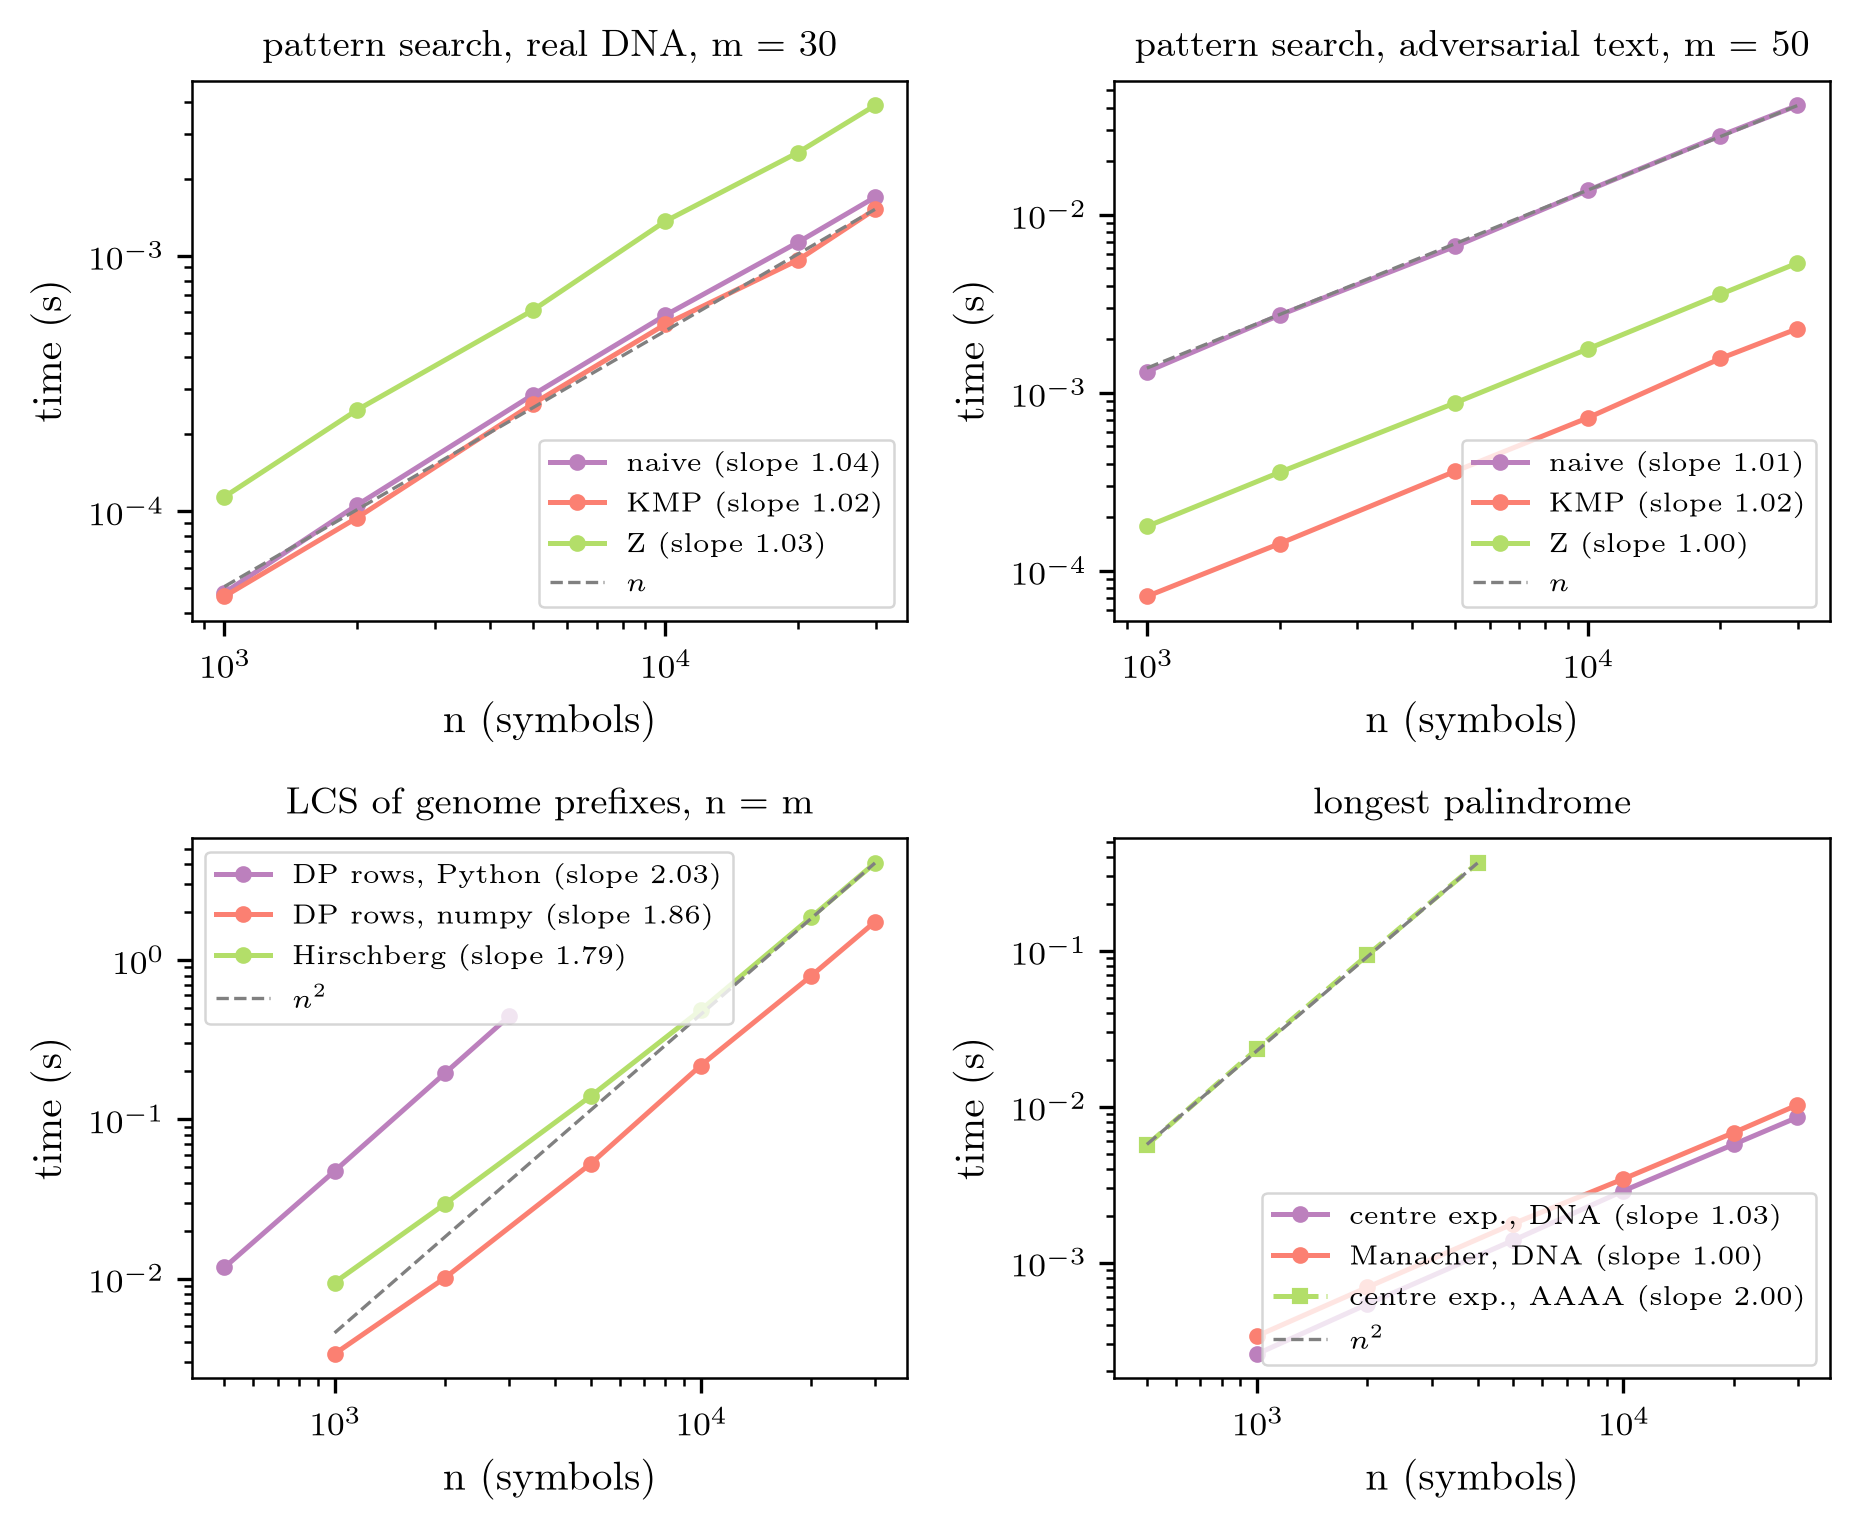
\includegraphics[width=0.8\textwidth]{fig_time_scaling}
    \caption{Running time against input size (log-log). Dashed lines are the theoretical growth anchored at the largest measurement; slopes in the legends are least-squares fits.}
    \label{fig:time}
\end{figure}

\ph{Explain Figure~\ref{fig:time} panel by panel. Search on real DNA: all three linear (slopes close to 1, Table~\ref{tab:complexity}); naive is not slower because a mismatch ends most alignments after one or two comparisons; Z is two to three times KMP because it builds and stores an array of $n + m + 1$ values while KMP keeps one pointer. Adversarial text: naive is still slope 1 in $n$ but 20 times slower than KMP, the factor $m = 50$ of the $O(nm)$ bound; KMP and Z unchanged. LCS: pure Python rows and numpy rows both have slope close to 2, quadratic as $O(nm)$ with $n = m$; Hirschberg has the same slope and costs about twice the numpy rows, the $2nm$ bound; the pure Python version reaches only $n = 3\,000$ in the time numpy needs for the full genomes. Palindromes: centre expansion linear on DNA (1.02) but quadratic on $A^n$ (2.00); Manacher linear on both.}

\begin{figure}[H]
    \centering
    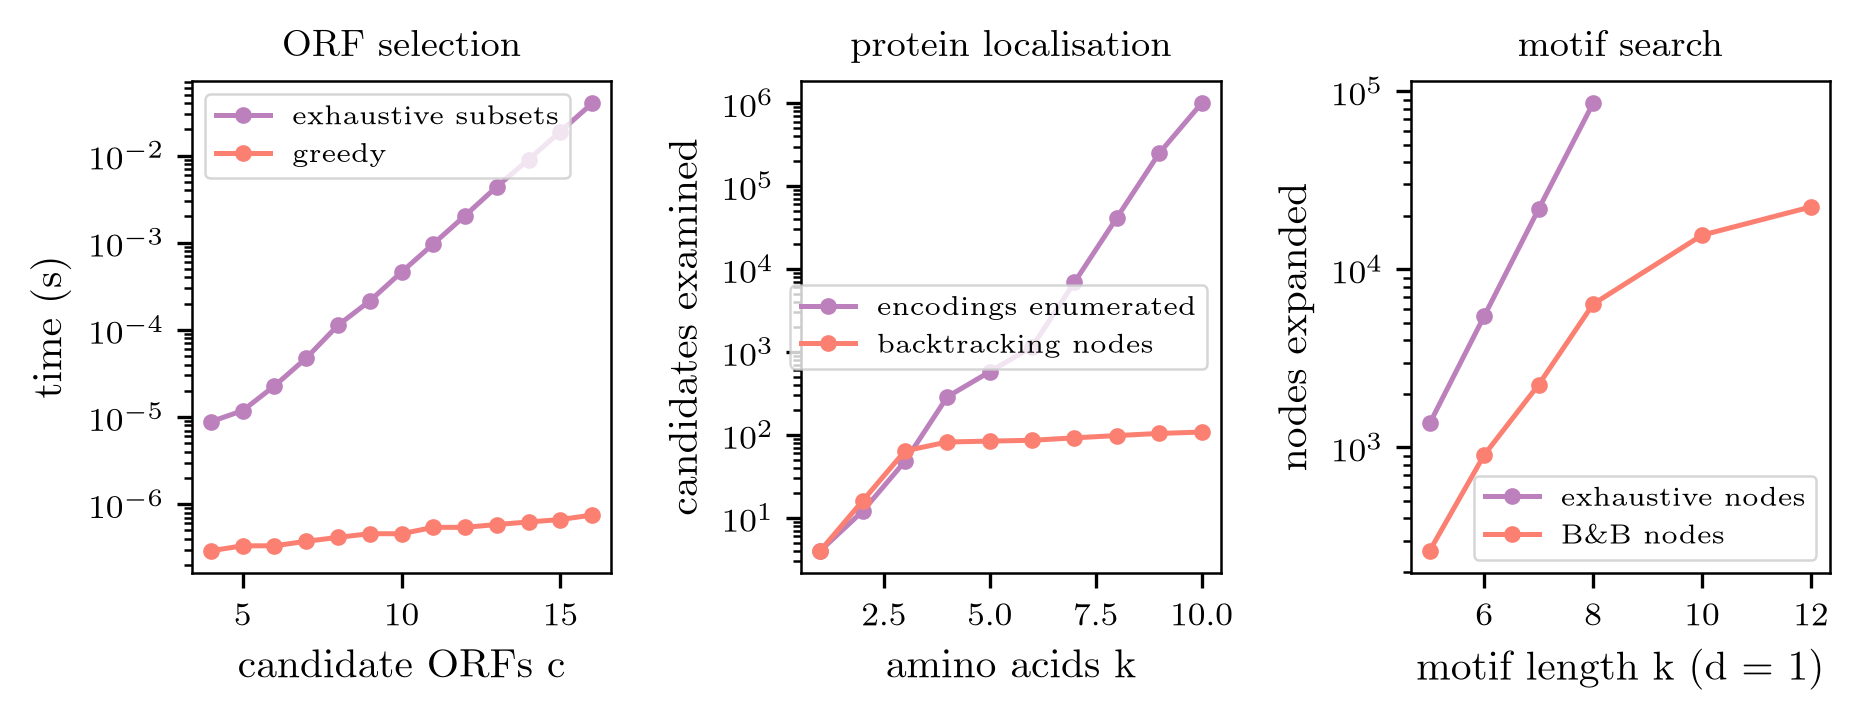
\includegraphics[width=0.85\textwidth]{fig_search_space}
    \caption{Search-space techniques against their baselines: exhaustive subsets versus greedy, encodings enumerated versus backtracking nodes, exhaustive versus branch-and-bound nodes.}
    \label{fig:search_space}
\end{figure}

\ph{Explain Figure~\ref{fig:search_space}. Exhaustive subset search doubles with every candidate while greedy is flat; enumerating encodings grows by the codon degeneracy at each amino acid (up to $10^6$ at $k = 10$) while backtracking stays near 100 nodes because after three amino acids the prefix pins down a single genome position; branch and bound expands about 7\% of the exhaustive nodes at $k = 8$ and keeps growing slowly to $k = 12$, where exhaustive search is no longer feasible.}
